\section{Analysis}
\label{sec:analysis}
This section will cover problem domain analysis, use case identification for the system to be developed, mapping of various requirements, and identifying potential constraints on the system. 

We start by identifying the basic requirements needed to develop networked traffic control for autonomous vehicles. The following 10 requirements will be considered in the analysis
\begin{enumerate}
    \item All of the controllers in the system must be able to communicate with one another and work together as a single, decentralized system.
    \item The controllers must be able to communicate with each other as well as other devices in the network.
    \item The system must be able to allow traffic authorities to monitor and adjust traffic signals.
    \item The system must follow standards that other users can use.
    \item The system must also be able to handle real-time data, make quick decisions, and manage traffic flow in real-time.
    \item The system must be able to schedule traffic at the intersection.
    \item The system should establish public transportation schedules and prioritize public transportation when necessary.
    \item The system should also have the capability to communicate with emergency vehicles.
    \item The system should provide emergency vehicles with priority access to the intersection.
    \item The system controller should be able to schedule pedestrian crossings.
\end{enumerate}
Based on the requirements above we can define the use case for the system.  
\subsection{System Use Case}
\label{subsec:use_case}
Based on the requirements above, we can define the use case for the networked traffic controller in Figure \ref{img:main_use_case}. We consider three main actors that will interact with the system: the administrator, the pedestrian, and the autonomous vehicle. The administrator can monitor the traffic. The pedestrian can use the system to request a crossing while the system ensures pedestrian safety. The system should optimize traffic flow and be able to dynamically adjust traffic signals. It should coordinate traffic at the intersection in real-time and avoid collisions between vehicles. It should encourage public transport and prioritize emergency vehicles.
\begin{figure}[ht]
    \centering
    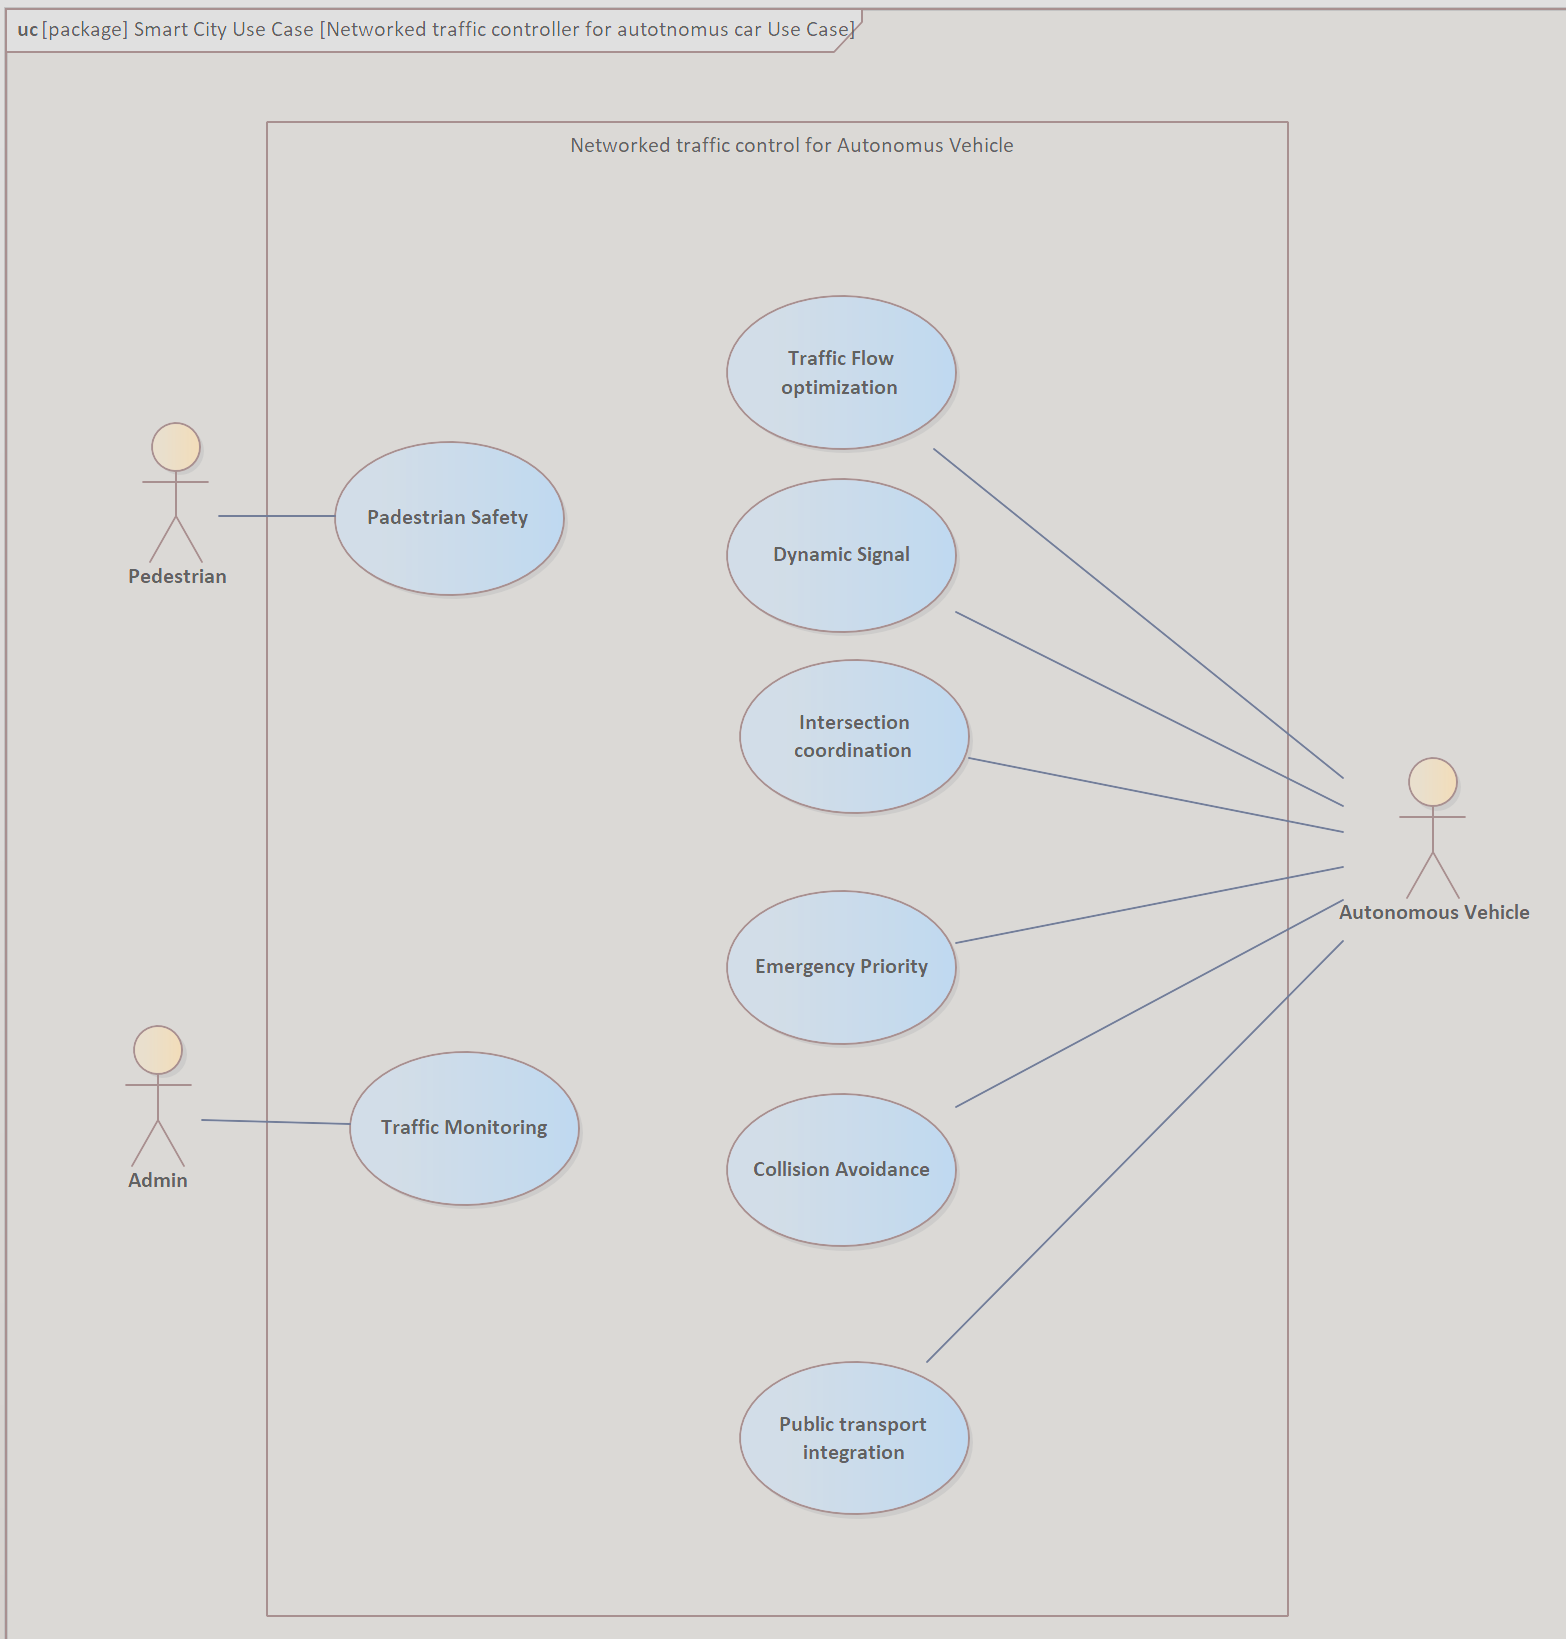
\includegraphics[width=0.5\textwidth]{images/main_use_case.png}
    \caption{Use Case Diagram}
    \label{img:main_use_case}
\end{figure}
